\documentclass[times, utf8, zavrsni]{fer}
\usepackage{booktabs}

\begin{document}

% TODO: Navedite broj rada.
\thesisnumber{123456}

\title{web aplikacija za predstavljanje portfelja programera}

\author{Mislav Vuletić}

\maketitle

% Ispis stranice s napomenom o umetanju izvornika rada. Uklonite naredbu \izvornik ako želite izbaciti tu stranicu.
% \izvornik

\zahvala{}

\tableofcontents

\chapter{Uvod}
\qquad Prilikom traženja posla prednost je ako se programer može predstaviti potencijalnom poslodavcu sa svim projektima u kojima je sudjelovao i programskom podrškom koju je razvio.
Često se za tu svrhu koriste LinkedIn ili Git stranice, odnosno druge vlastite Web stranice programera.
Učinkovito predstavljanje može se postići uz pomoć jedne stranice koja će omogućavati pregled projekata kroz Git alate, sadržavati linkove na aktivne projekte te omogućiti međusoban kontakt programera i poslodavca putem korisničkog sučelja.

\chapter{Arhitektura}
Klase su podjeljene na...

\begin{figure}[htb]\centering
				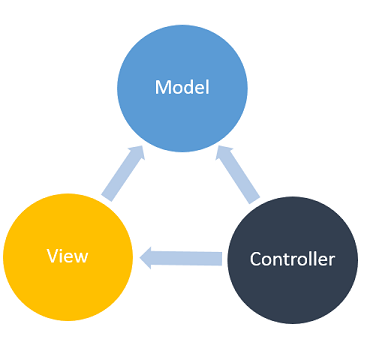
\includegraphics[width=10cm]{images/mvc.png}
				\caption{MVC struktura}
				\label{fig:mvc}
\end{figure}


\chapter{Zaključak}
Zaključak.

\bibliography{literatura}
\bibliographystyle{fer}

\begin{sazetak}
Sažetak na hrvatskom jeziku.

\kljucnerijeci{Ključne riječi, odvojene zarezima.}
\end{sazetak}

\engtitle{Software Developer Portfolio Web Application}
\begin{abstract}
Abstract.

\keywords{Keywords.}
\end{abstract}

\end{document}
